%\textcolor{red}{\hrulefill \textsc{Unfinished Section}\hrulefill}  \\
One of the more interesting developments in this field in recent years is in the space  of \emph{Analysis Preservation} and the closely related \emph{Recasting of Analyses}.
The nominal way of preserving a scientific analysis such that it is effectively reproducible is by way of the tried and true method of publishing a paper, and, perhaps, a linked collection of relevant data tables from that analysis. 
Now for many (most) fields this is still very much sufficient.
But for anyone familiar with experiments such as \ATLAS whose collaborations consist of thousands of scientists, hundreds of pieces of evolving software, hardware, and working point recommendations, the actual reproducibility of a single analysis becomes intractable.
The resulting paper would ultimately become a list of various versions of internal pieces of software and this often legitimate information is lost in the final journal version of the paper because there is just too much information contained in the full analysis to be published.
Fortunately as our experiments grow in complexity our technology grows too in power and capability.
In recent years there have been tremendous strides in general software and computing technology that allows for, on a user level, the ability to capture entire computing environments and analysis workflows in a relatively lightweight manner that can produce exact results seen in the the published paper.
What we effectively have then is a custom piece of software built for a singular high energy physics analysis that can produce paper quality results with a single command. 
\Cern's specific efforts towards these goals take form in the \CERN ~Analysis Preservation (CAP)~\cite{CAP:2021} service and the REANA (\textbf{Re}usable \textbf{Ana}lysis) platform~\cite{reana:2021}.
While ATLAS has it's own internal framework RECAST~\cite{recast:2021}, which was developed closely along side REANA (and is compatible syntactically with only a \href{https://recast-docs.web.cern.ch/recast-docs/using/#set-up-environment-variables-to-access-reanacernch-cluster}{few changes}).

\subsection{Analysis Preservation for the Trilepton Resonance Search}
%While some of this technology has been available and widely used in industry it is only just in the past few years become a consideration for most analysers in this field.
The process of preserving an analysis will be detailed in the context of this trilepton resonance search.

\subsubsection{Preserving the Data}
Actual data preservation is nothing new, raw data is of course preserved on tape at CERN and on disk at several tier 1 sites. 
But what people usually mean when talking about preserving data is the processed and analyzed data, i.e. the statistical results and supporting data.
The efforts with this type of preservation for scattering experiments dates back to around 1975 with the advent of the Durham HepData Project, a database for results from particle physics experiments. 
The modern version was released in 2016 as \mbox{HEPData}~\cite{hepdata:2021} as a well indexed HEP results database with intuitive responsive data table visualizations. 
Whereas in the early days the project was driven from within in order to collect data from the experimentalists, additions to the database are now almost entirely community driven and is now regularly updated with results from the experimentalists themselves with support and review from the HEPData project.
%The types of data that can exist in this space is public,
The HEPData space for this trilepton resonance search can be found here \href{https://www.hepdata.net/record/ins1831992}{https://www.hepdata.net/record/ins1831992}

\subsubsection{Preserving the Analysis}
To preserve the actual analysis, in the most literal sense, the full underlying codebase that produces the final public results must be preserved.
This can be as easy as just maintaining one's analysis code on a version controlled repository.
But where this runs into problems almost immediately is the tremendous burden on the developers to actually make the often incredibly complicated codebase usable, and understandable to future users (non-developers). 
This not only entails a necessarily detailed explanation of how to use the code but also an exhaustive list of its dependencies and libraries to ensure that it even works many years down the line, and you effectively have become a full fledged software developer. 
Fortunately, there is a nice way around a lot of this.
A computational tool known as OS-virtualization by way of containers, most commonly referred to as just ``containers.''
Containers behave like a the more familiar virtual machine in many ways. 
The key difference from a virtual machine is that rather than creating a whole virtual operating system, containers need only the individual components required to operate the software of interest.
This gives a significant performance boost and reduces the size of the application.
They also operate much faster, as unlike traditional virtualization the process is essentially running natively on its host, just with an additional layer of protection around it.
Containers have existed in some form for over a decade but really only gained traction in the computational world in 2013 when Docker released their containerization platform.
Open-source and well maintained, Docker provided their own containers known as docker images, a registry to host those images, and created the Dockerfile, a simple file that contains all the commands to assemble an image. 
This combination made it incredibly easy to create images that anyone could run on any machine.
To this end \ATLAS has been Dockerizing its analysis platform Athena \cite{Athena:2021} (amongst an increasing number of other pieces of relevant software) since 2017, providing a large number of releases (stable versions of the software) readily available for use.
Automatic containerization then becomes shockingly simple by way of continuous integration by including the aforementioned \emph{Dockerfile} in your version controlled repository.
For this analysis it looks like the following:
\begin{lstlisting}[
backgroundcolor=\color{bkgcolor},
commentstyle=\color{comments},
rulecolor=\color{bkgcolor},
stringstyle=\color{string},
language=bash, 
numbers=left, 
numbersep=5pt,
breaklines=true,  
basicstyle=\linespread{1.2}\ttfamily\scriptsize\color{white},  
showspaces=false, 
showstringspaces=false, 
showtabs=false,
keywordstyle=\color{var}, 
numberstyle=\tiny\color{codegray},
columns=fullflexible,
xleftmargin=0.5cm,
frame=tlbr,
framesep=4pt,
framerule=0pt
]
FROM atlas/analysisbase:21.2.78
ADD . /analysis/
WORKDIR /analysis/build
RUN source /home/atlas/release_setup.sh &&\ 
    sudo chown -R atlas /analysis &&\
    echo "ls"; ls &&\
    echo "ls ../"; ls ../ &&\
    echo "ls ../patch"; ls ../patch &&\
    source ../patch/apply_patch.sh &&\
    cmake ../source &&\
    make -j4 &&\ 
    bash -c "cd ../source/HistFitter && \
    . setup.sh && cd src && make"
USER root
RUN sudo usermod -aG root atlas # Replace 'atlas' with the default user in your analysis image, if different
USER atlas. 
\end{lstlisting}

Where in the first line is the Docker image of the specific release of the internal ATLAS software used for this analysis, then the remainder of the lines builds and sets up this release as well as all the local code contained in the repository in which the Dockerfile exists (and also applies a small very specific patch to some code contained in a submodule).
This produces a new Docker image every time code is pushed to the repository using continuous integration.

\subsubsection{Workflow Authoring}
The next step known as \emph{workflow authoring} and it effectively specifies a series of commands with a set of configurable inputs that will allow an end user to easily run the full analysis code that results in statistical statements ($p$-values/CLs values).
Using the Markup type language YAML (or yadage), a human readable data-serialization language, external data file inputs can be passed in as variables, processed in one step, and have the step's output fed into the next step and so on.
The first step in our framework can be seen below as an example of what this actually looks like in code, and can also be seen illustrated in Figure~\ref{fig:rpvthreel:workflow} as the first dashed line box as part of the full workflow.
\begin{lstlisting}[
backgroundcolor=\color{bkgcolor},
commentstyle=\color{comments},
rulecolor=\color{bkgcolor},
stringstyle=\color{string},
language=bash, 
numbers=left, 
numbersep=5pt,
breaklines=true,  
basicstyle=\linespread{1.2}\ttfamily\scriptsize\color{white},  
showspaces=false, 
showstringspaces=false, 
showtabs=false,
keywordstyle=\color{var}, 
numberstyle=\tiny\color{codegray},
columns=fullflexible,
xleftmargin=0.5cm,
frame=tlbr,
framesep=4pt,
framerule=0pt
]
daod_to_ntup_mc16ade:
  process:
    process_type: interpolated-script-cmd
    interpreter: bash
    script: |
      source /recast_auth/getkrb.sh
      source /home/atlas/release_setup.sh
      source /analysis/build/*/setup.sh
      cd /analysis
      python ./source/xAODAnaHelpers/scripts/xAH_run.py -f --scanXRD --inputList --files {input_file_mc16a} --submitDir {submitDir_mc16a} --config source/BMinusLCharginoAnalysis/data/config_BMinusLChargino_AFII_mc16a.py direct
      python source/BMinusLCharginoAnalysis/scripts/appendParsedNames.py --filelistpath {input_file_mc16a} --outputTrees {submitDir_mc16a}/data-tree/
      python ./source/xAODAnaHelpers/scripts/xAH_run.py -f --scanXRD --inputList --files {input_file_mc16d} --submitDir {submitDir_mc16d} --config source/BMinusLCharginoAnalysis/data/config_BMinusLChargino_AFII_mc16d.py direct
      python source/BMinusLCharginoAnalysis/scripts/appendParsedNames.py --filelistpath {input_file_mc16d} --outputTrees {submitDir_mc16d}/data-tree/
      python ./source/xAODAnaHelpers/scripts/xAH_run.py -f --scanXRD --inputList --files {input_file_mc16e} --submitDir {submitDir_mc16e} --config source/BMinusLCharginoAnalysis/data/config_BMinusLChargino_AFII_mc16e.py direct
      python source/BMinusLCharginoAnalysis/scripts/appendParsedNames.py --filelistpath {input_file_mc16e} --outputTrees {submitDir_mc16e}/data-tree/
      mkdir {submitDir_all}
      cp {submitDir_mc16a}/data-tree/* {submitDir_all}/
      cp {submitDir_mc16d}/data-tree/* {submitDir_all}/
      cp {submitDir_mc16e}/data-tree/* {submitDir_all}/
      ls {submitDir_all}
  publisher:
    publisher_type: interpolated-pub
    publish:
      ntup_mc16ade: '{submitDir_all}'
    glob: true
  environment:
    environment_type: docker-encapsulated
    image: gitlab-registry.cern.ch/atlassusy-bminusl/bminuslcharginoanalysis
    imagetag: master
    resources:
      - kubernetes_uid: 500
      - kerberos: true
\end{lstlisting}
Where you can see in line \texttt{28} the Docker image that was created by the Dockerfile shown previously is specified.
Then lines \texttt{6-20} are the actual commands being run within this image environment which takes a very familiar form: set up environment with some scripts + run high level python script with various options.
All things appearing in curly brackets (braces) are variable.
\begin{figure}[ht]
  \begin{center}
    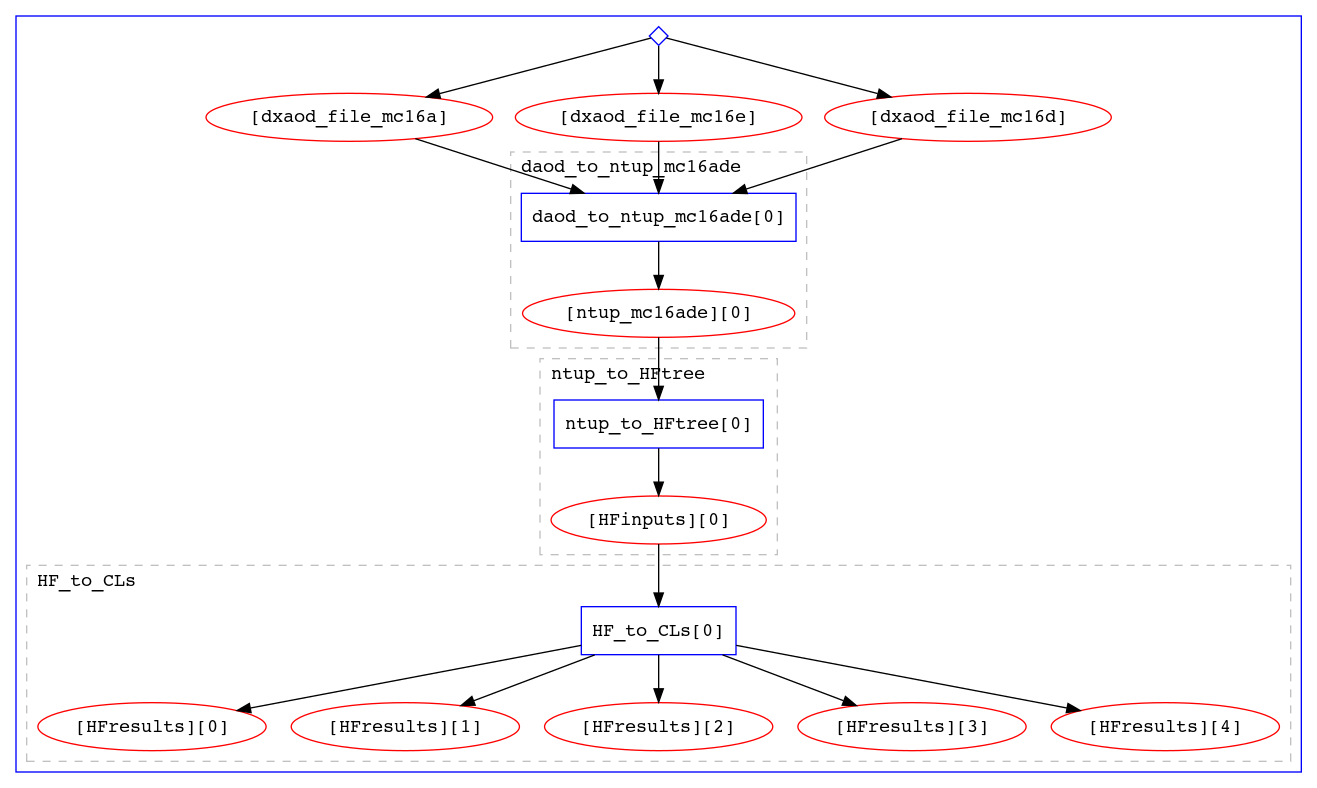
\includegraphics[width=0.98\textwidth]{figs/rpvthreel/yadage_workflow_instance.png}
  \end{center}
  \caption{Diagrammatic illustration of full step-by-step analysis workflow.
  Explicit steps are \texttt{daod\_to\_ntup\_mc16ade}, \texttt{ntup\_to\_HFtree}, and \texttt{HF\_to\_CLs} with inputs \texttt{dxaod\_file\_mc16a}, \texttt{dxaod\_file\_mc16d}, and \texttt{dxaod\_file\_mc16e} representing the three MC campaigns used in the analysis.}
  \label{fig:rpvthreel:workflow}
\end{figure}
From Figure~\ref{fig:rpvthreel:workflow} we also see the general structure of the analysis workflow, which is as follows:
\begin{itemize}
    \item \texttt{daod\_to\_ntup\_mc16ade} : Step taking data from a relatively general form, \texttt{DOAD}, and computing high level analysis quantities, creating a smaller data type containing only relevant analysis information. 
    \item \texttt{ntup\_to\_HFtree} : Further slimming of data and reformatting for use in the statistical tool \texttt{HistFitter}.
    \item \texttt{HF\_to\_CLs} : Running the statistical machinery (\texttt{HistFitter}) that outputs the final statistical results.
\end{itemize}

%\subsection{Recasting the trilepton resonance search}
%\textcolor{red}{\hrulefill \textsc{Unfinished Section}\hrulefill}  \\